% Rebuild: xelatex -no-pdf -interaction=nonstopmode finger-tree-3.tex
%          dvisvgm --no-fonts --exact-bbox finger-tree-3.xdv -o finger-tree-3.svg
\def\pgfsysdriver{pgfsys-dvisvgm.def}
\documentclass[tikz,border=4pt]{standalone}
\usetikzlibrary{arrows.meta,backgrounds}
\begin{document}
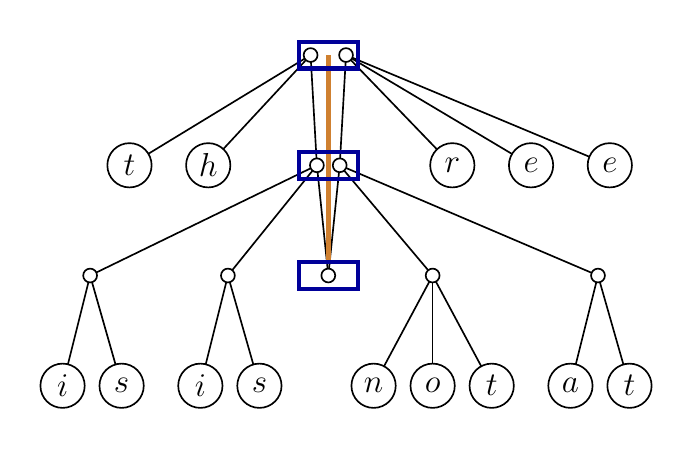
\begin{tikzpicture}[background rectangle/.style={fill=white},show background rectangle,x=1cm,y=1cm,line width=.6pt,
  internal/.style={circle,draw,fill=white,inner sep=0pt,minimum size=5pt},
  leaf/.style={circle,draw,fill=white,inner sep=0pt,minimum size=16pt,font=\large}]
\coordinate (topL) at (3.4,4.2);
\coordinate (topR) at (3.85,4.2);
\coordinate (midL) at (3.48,2.8);
\coordinate (midR) at (3.77,2.8);
\coordinate (root) at (3.625,1.4);
\coordinate (g1) at (0.6,1.4);
\coordinate (g2) at (2.35,1.4);
\coordinate (g3) at (4.95,1.4);
\coordinate (g4) at (7.05,1.4);
\coordinate (l0) at (1.1,2.8);
\coordinate (l1) at (2.1,2.8);
\coordinate (l11) at (5.2,2.8);
\coordinate (l12) at (6.2,2.8);
\coordinate (l13) at (7.2,2.8);
\coordinate (l2) at (0.25,0);
\coordinate (l3) at (1,0);
\coordinate (l4) at (2,0);
\coordinate (l5) at (2.75,0);
\coordinate (l6) at (4.2,0);
\coordinate (l7) at (4.95,0);
\coordinate (l8) at (5.7,0);
\coordinate (l9) at (6.7,0);
\coordinate (l10) at (7.45,0);
\draw (topL) -- (l0);
\draw (topL) -- (l1);
\draw (topL) -- (midL);
\draw (topR) -- (l11);
\draw (topR) -- (l12);
\draw (topR) -- (l13);
\draw (topR) -- (midR);
\draw (midL) -- (g1);
\draw (midL) -- (g2);
\draw (midL) -- (root);
\draw (midR) -- (root);
\draw (midR) -- (g3);
\draw (midR) -- (g4);
\draw (g1) -- (l2);
\draw (g1) -- (l3);
\draw (g2) -- (l4);
\draw (g2) -- (l5);
\draw (g3) -- (l6);
\draw (g3) -- (l7);
\draw (g3) -- (l8);
\draw (g4) -- (l9);
\draw (g4) -- (l10);
\node[internal] at (topL) {};
\node[internal] at (topR) {};
\node[internal] at (midL) {};
\node[internal] at (midR) {};
\node[internal] at (root) {};
\node[internal] at (g1) {};
\node[internal] at (g2) {};
\node[internal] at (g3) {};
\node[internal] at (g4) {};
\node[leaf] at (l0) {$t$};
\node[leaf] at (l1) {$h$};
\node[leaf] at (l11) {$r$};
\node[leaf] at (l12) {$e$};
\node[leaf] at (l13) {$e$};
\node[leaf] at (l2) {$i$};
\node[leaf] at (l3) {$s$};
\node[leaf] at (l4) {$i$};
\node[leaf] at (l5) {$s$};
\node[leaf] at (l6) {$n$};
\node[leaf] at (l7) {$o$};
\node[leaf] at (l8) {$t$};
\node[leaf] at (l9) {$a$};
\node[leaf] at (l10) {$t$};

% Each blue box is one level of the finger tree; brown marks its spine.
\draw[brown!75!orange,line width=2pt] (3.625,4.2) -- (3.625,1.55);
\foreach \y in {4.2,2.8,1.4}
  \draw[blue!60!black,line width=1.5pt] (3.25,\y-.17) rectangle (4,\y+.17);
\end{tikzpicture}
\end{document}
